Unless stated otherwise, ``error'' means the time-averaged logical error over
rounds 1--50. It is the most precise paired statistic and does not saturate.
$P_L(50)$ is reported alongside it. A dagger ($^\dagger$) marks fewer than 10
observed errors, and ``$<x$'' is the 95\% upper bound $3/N$ when none were
observed.

%----------------------------------------
\subsection{E1: main comparison at the nominal point}

\begin{figure}[H]
\centering
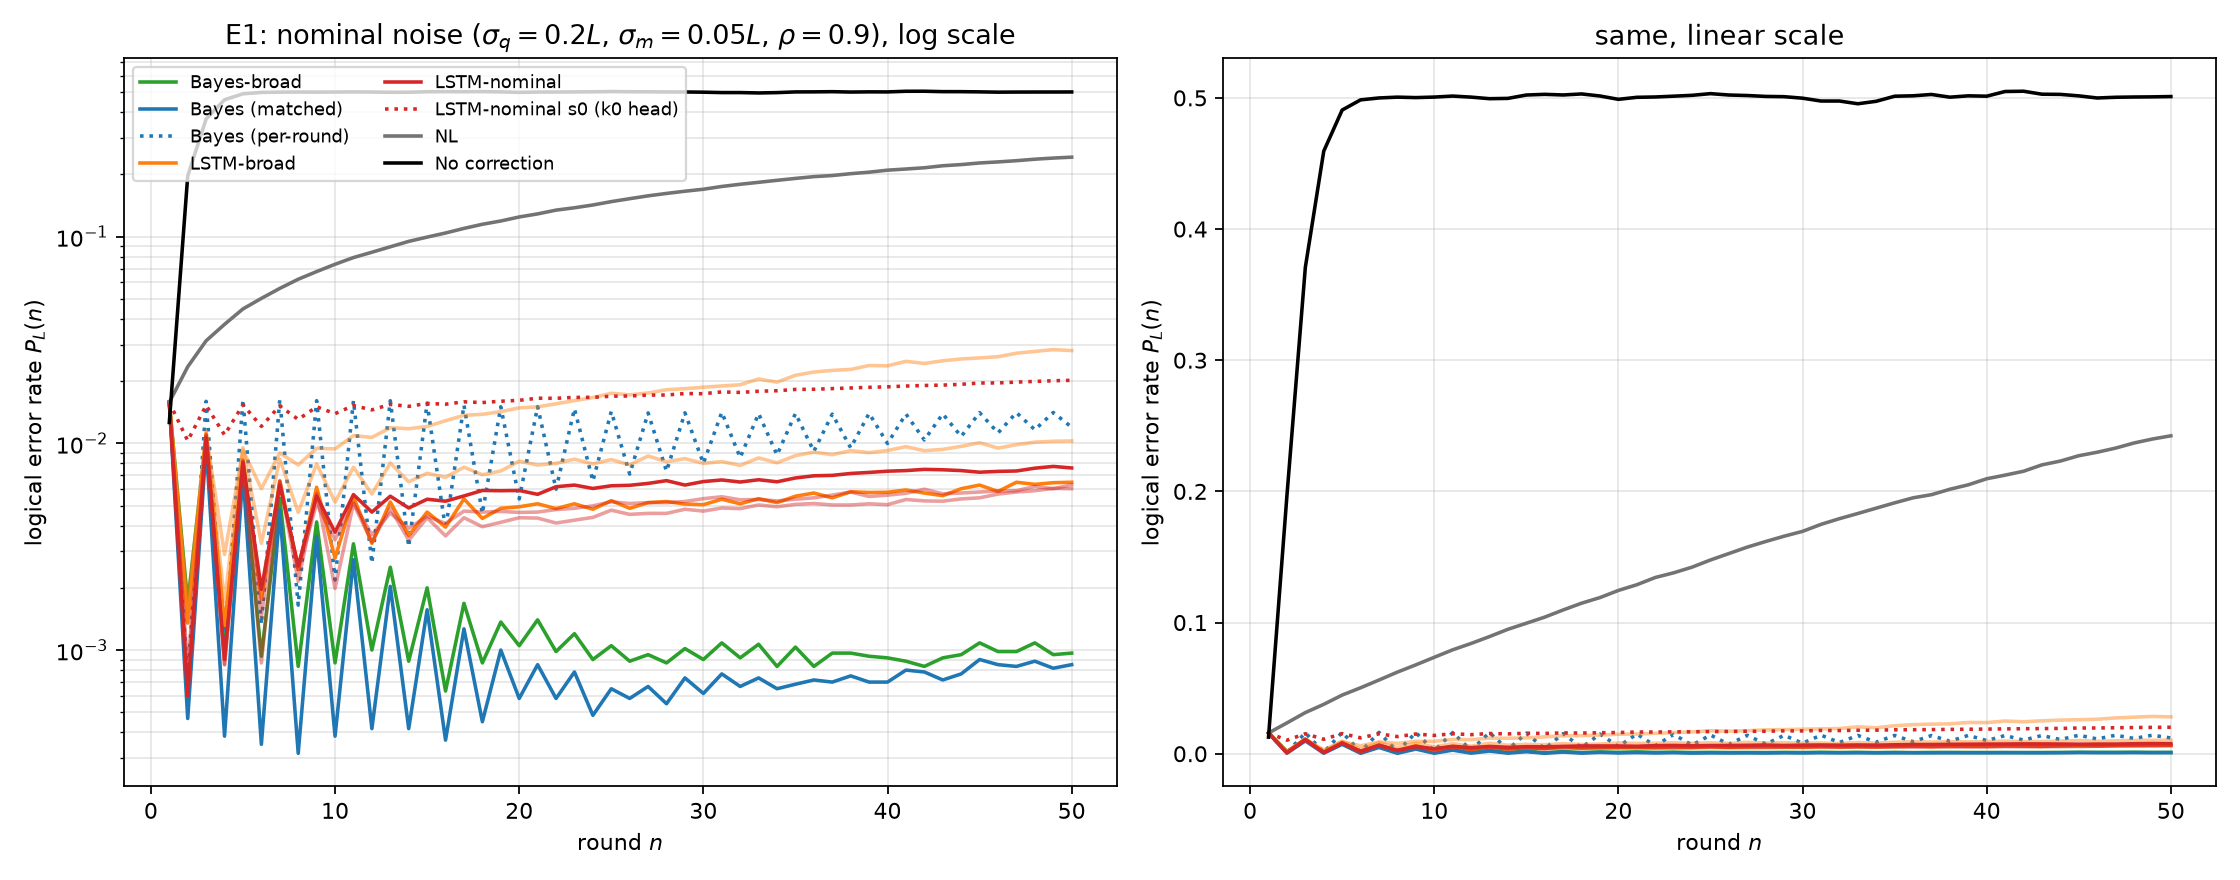
\includegraphics[width=\textwidth]{E1_ler_vs_round.png}
\caption{E1: logical error rate after each round at $\sigma_q=0.2L$,
$\sigma_m=0.05L$, $\rho=0.9$ (\EoneBayesTrials{} trials, common noise).
Faint lines are the individual LSTM seeds.}
\label{fig:e1}
\end{figure}

\begin{table}[H]
\centering\small
\begin{tabular}{lrrrr}
\toprule
Decoder & $P_L(10)$ & $P_L(50)$ & time-avg.\ error & paired diff.\ vs Bayes \\
\midrule
No correction & $0.501$ & $0.501$ & $0.481$ & $+0.480$ {\scriptsize($\pm1\!\times\!10^{-3}$)} \\
NL & $0.073$ & $0.242$ & $0.144$ & $+0.142$ {\scriptsize($\pm2\!\times\!10^{-3}$)} \\
Bayes (matched) & $3.8\!\times\!10^{-4}$ & $8.5\!\times\!10^{-4}$ & $1.5\!\times\!10^{-3}$ & -- \\
Bayes (per-round) & $2.2\!\times\!10^{-3}$ & $0.012$ & $0.011$ & $+9.2\!\times\!10^{-3}$ {\scriptsize($\pm6\!\times\!10^{-4}$)} \\
Bayes-broad & $8.7\!\times\!10^{-4}$ & $9.7\!\times\!10^{-4}$ & $1.9\!\times\!10^{-3}$ & $+3.7\!\times\!10^{-4}$ {\scriptsize($\pm1\!\times\!10^{-4}$)} \\
\textbf{LSTM-nominal (mean of seeds)} & $3.0\!\times\!10^{-3}$ & $6.6\!\times\!10^{-3}$ & $5.5\!\times\!10^{-3}$ & $+4.0\!\times\!10^{-3}$ {\scriptsize($\pm4\!\times\!10^{-4}$)} \\
LSTM-nominal s0 & $3.7\!\times\!10^{-3}$ & $7.6\!\times\!10^{-3}$ & $6.3\!\times\!10^{-3}$ & $+4.8\!\times\!10^{-3}$ {\scriptsize($\pm4\!\times\!10^{-4}$)} \\
LSTM-nominal s1 & $3.4\!\times\!10^{-3}$ & $6.3\!\times\!10^{-3}$ & $5.3\!\times\!10^{-3}$ & $+3.8\!\times\!10^{-3}$ {\scriptsize($\pm4\!\times\!10^{-4}$)} \\
LSTM-nominal s2 & $2.0\!\times\!10^{-3}$ & $6.0\!\times\!10^{-3}$ & $4.9\!\times\!10^{-3}$ & $+3.4\!\times\!10^{-3}$ {\scriptsize($\pm4\!\times\!10^{-4}$)} \\
LSTM-nominal s0 (per-round head) & $0.014$ & $0.020$ & $0.017$ & $+0.015$ {\scriptsize($\pm9\!\times\!10^{-4}$)} \\
\textbf{LSTM-broad (mean of seeds)} & $5.8\!\times\!10^{-3}$ & $0.015$ & $0.010$ & $+8.7\!\times\!10^{-3}$ {\scriptsize($\pm4\!\times\!10^{-4}$)} \\
LSTM-broad s0 & $2.8\!\times\!10^{-3}$ & $6.5\!\times\!10^{-3}$ & $5.4\!\times\!10^{-3}$ & $+3.9\!\times\!10^{-3}$ {\scriptsize($\pm4\!\times\!10^{-4}$)} \\
LSTM-broad s1 & $9.4\!\times\!10^{-3}$ & $0.028$ & $0.017$ & $+0.016$ {\scriptsize($\pm7\!\times\!10^{-4}$)} \\
LSTM-broad s2 & $5.2\!\times\!10^{-3}$ & $0.010$ & $8.2\!\times\!10^{-3}$ & $+6.6\!\times\!10^{-3}$ {\scriptsize($\pm4\!\times\!10^{-4}$)} \\
\bottomrule
\end{tabular}
\caption{E1 at the nominal point. The paired difference is the mean per-trial
difference in time-averaged error from matched Bayes, with its 2-SE
uncertainty. For the seed means the uncertainty shown is that of seed~0.}
\label{tab:e1}
\end{table}

Memory changes the picture completely (Figure~\ref{fig:e1},
Table~\ref{tab:e1}):
\begin{itemize}
  \item \textbf{Nearest lattice} accumulates errors steadily and reaches
    $P_L(50)=\EoneNLLERfifty$.
  \item \textbf{Matched Bayes} reaches $P_L(50)=\EoneBayesLERfifty$, which is
    \EoneBayesEvents{} errors in \EoneBayesTrials{} trials. Its time-averaged
    error is \EoneGain{} times smaller than NL's.
  \item \textbf{Bayes-broad} gets within about 25\% of matched Bayes without
    knowing the parameters ($\EoneBayesBroadMean$ against $\EoneBayesMean$).
  \item \textbf{LSTM-nominal} is trained at this exact point. It reaches a
    time-averaged error of $\EoneLSTMnomMean$, which is \EoneLSTMoverBayes{}
    times that of matched Bayes but still about 26 times better than NL. The
    three seeds lie within about 30\% of each other (3.3--4.2 times matched
    Bayes), a much smaller spread than for the broad seeds.
  \item \textbf{LSTM-broad} reaches $\EoneLSTMbroadMean$ on average, with a
    large spread between seeds: seed~0 matches LSTM-nominal and seed~1 is
    3 times worse. All three broad models finished their full 40-epoch
    schedule, and their validation losses differ little (Table~\ref{tab:training}).
    The spread therefore reflects how differently models trained on the whole
    box handle this particular corner of it, not undertraining.
\end{itemize}

Both ablations show that revising past decisions matters. Bayes restricted to
per-round decisions has error $\EoneBayesPRMean$, about 7 times worse than
full Bayes. The LSTM's per-round head ($k=0$) has error $\EoneLSTMkzeroMean$,
about 2.7 times worse than its cumulative head. Section~\ref{sec:why} explains
the zig-zag in the early rounds.

%----------------------------------------
\subsection{E2: stronger correlation}

\begin{figure}[H]
\centering
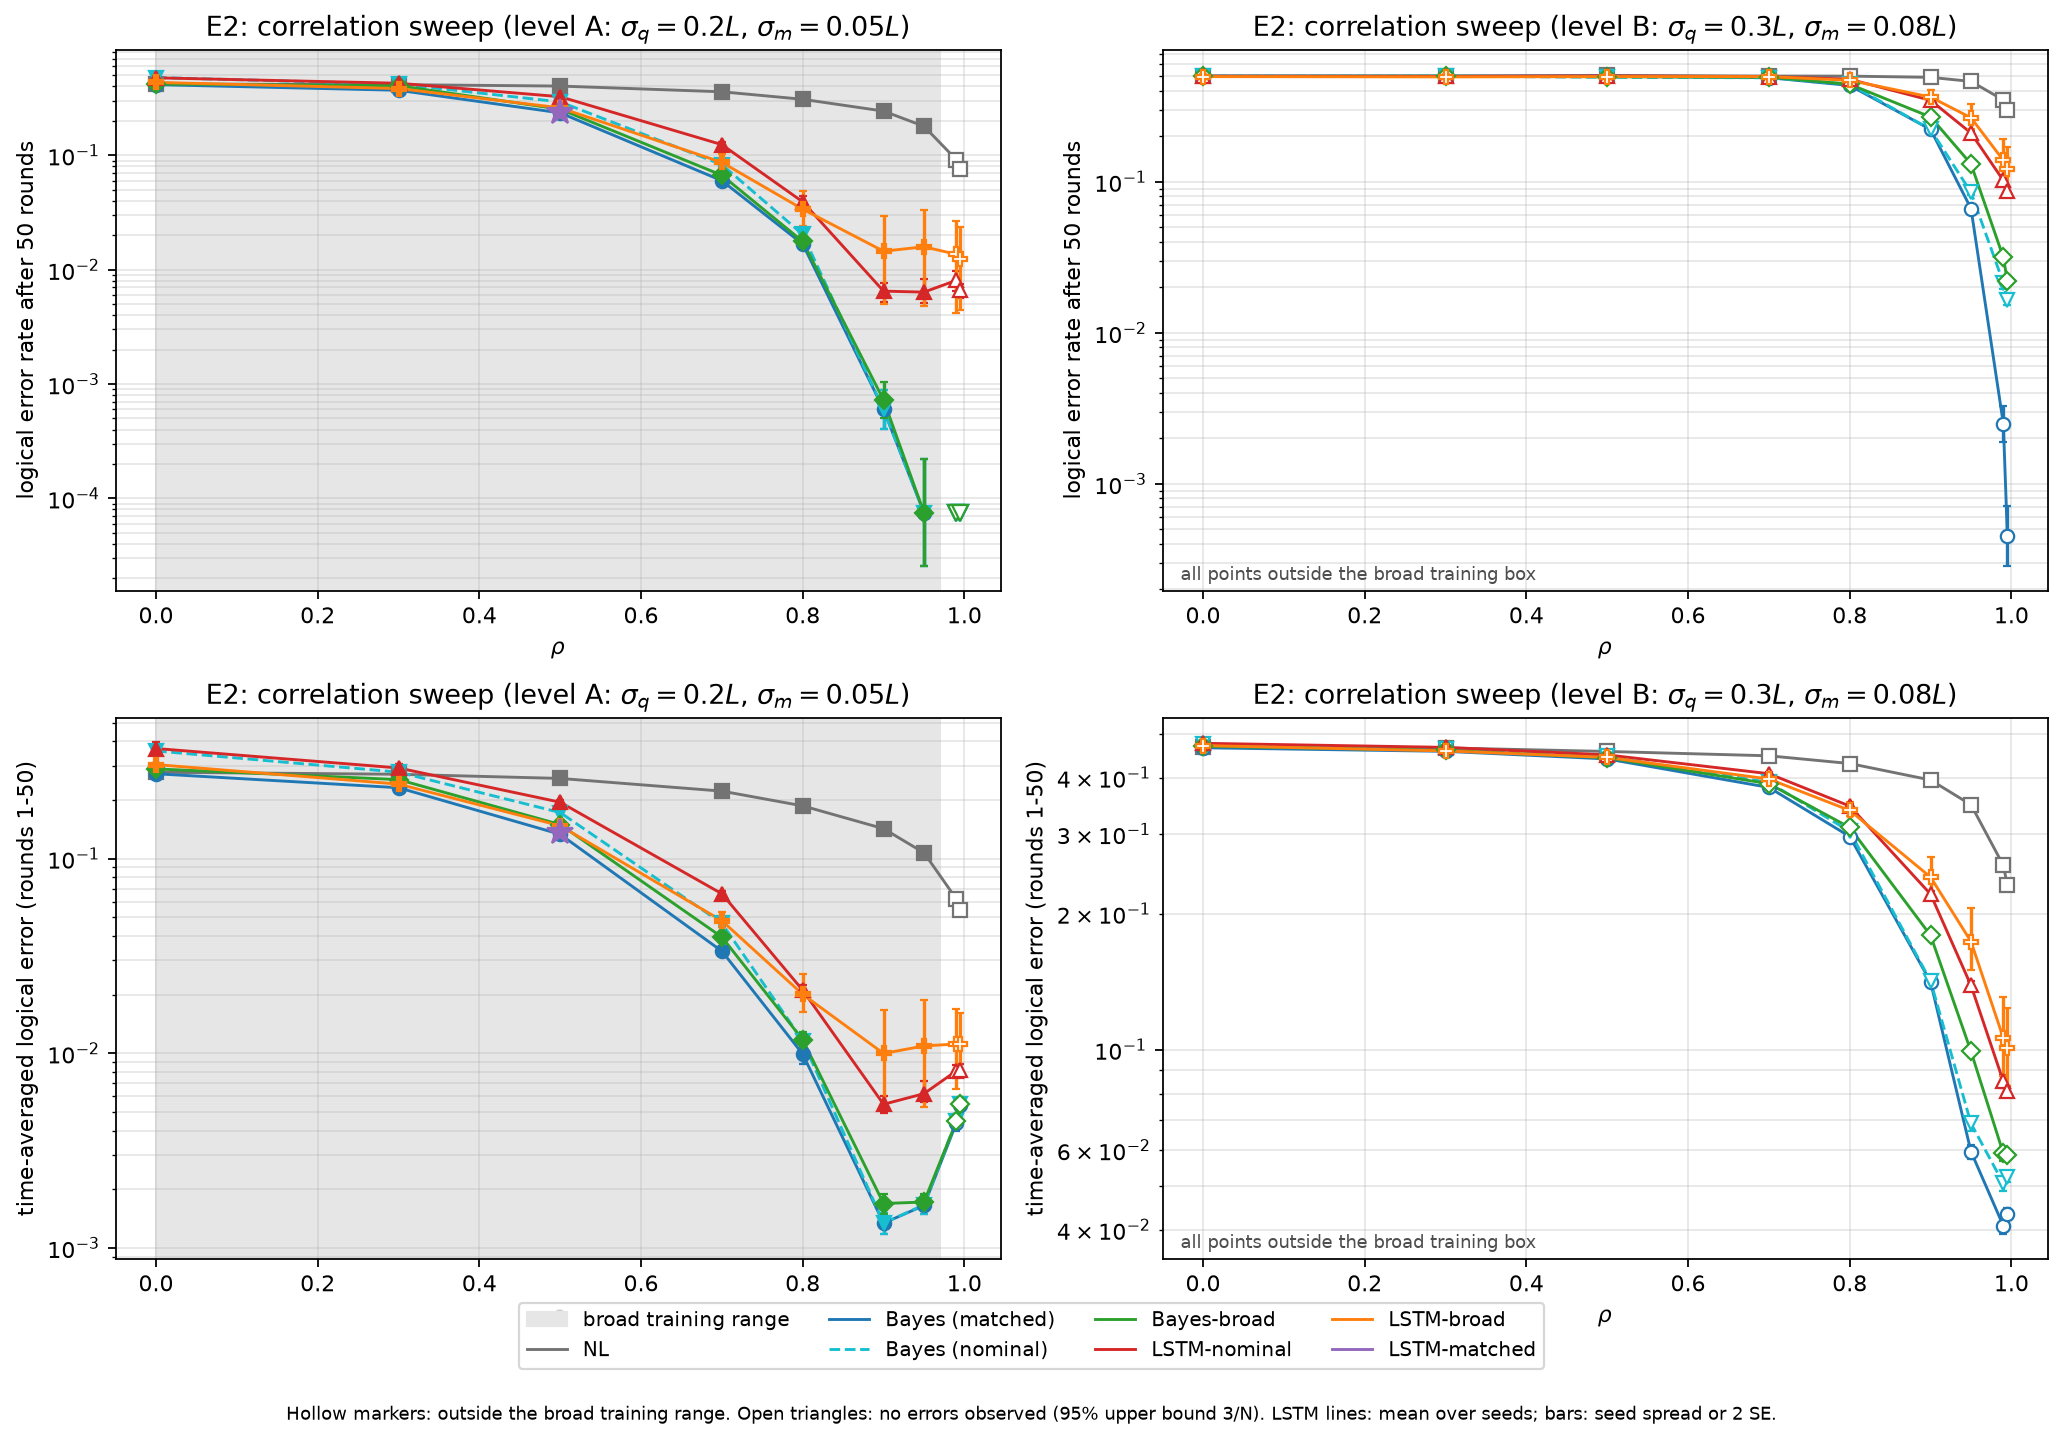
\includegraphics[width=\textwidth]{E2_rho_sweep.png}
\caption{E2: correlation sweep at two noise levels. Top: $P_L(50)$. Bottom:
time-averaged error. The shaded band is the $\rho$ range of the broad
training box. At level~B, $\sigma_q=0.3L$ lies outside the box
($\sigma_m=0.08L$ sits at its upper edge), so every point there is out of
distribution for both broad decoders.}
\label{fig:e2}
\end{figure}

\begin{table}[H]
\centering\small
\resizebox{\textwidth}{!}{\begin{tabular}{lrrrrrrr}
\toprule
$\rho$ & NL & Bayes (matched) & Bayes (nominal) & Bayes-broad & LSTM-nominal & LSTM-broad & LSTM-matched \\
\midrule
0.0 & $0.278$ & $0.273$ & $0.357$ & $0.289$ & $0.368$ & $0.304$ & -- \\
0.3 & $0.271$ & $0.231$ & $0.278$ & $0.255$ & $0.292$ & $0.241$ & -- \\
0.5 & $0.258$ & $0.133$ & $0.172$ & $0.150$ & $0.195$ & $0.147$ & $0.136$ \\
0.7 & $0.222$ & $0.033$ & $0.047$ & $0.040$ & $0.066$ & $0.048$ & -- \\
0.8 & $0.187$ & $9.9\!\times\!10^{-3}$ & $0.012$ & $0.012$ & $0.021$ & $0.020$ & -- \\
0.9 & $0.142$ & $1.3\!\times\!10^{-3}$ & $1.3\!\times\!10^{-3}$ & $1.7\!\times\!10^{-3}$ & $5.5\!\times\!10^{-3}$ & $10.0\!\times\!10^{-3}$ & -- \\
0.95 & $0.107$ & $1.6\!\times\!10^{-3}$ & $1.7\!\times\!10^{-3}$ & $1.7\!\times\!10^{-3}$ & $6.2\!\times\!10^{-3}$ & $0.011$ & -- \\
0.99 & $0.062$ & $4.4\!\times\!10^{-3}$ & $4.5\!\times\!10^{-3}$ & \textit{$4.5\!\times\!10^{-3}$} & $8.1\!\times\!10^{-3}$ & \textit{$0.011$} & -- \\
0.995 & $0.054$ & $5.4\!\times\!10^{-3}$ & $5.5\!\times\!10^{-3}$ & \textit{$5.5\!\times\!10^{-3}$} & $8.2\!\times\!10^{-3}$ & \textit{$0.011$} & -- \\
\bottomrule
\end{tabular}}
\\[4pt]
\resizebox{\textwidth}{!}{\begin{tabular}{lrrrrrrr}
\toprule
$\rho$ & NL & Bayes (matched) & Bayes (nominal) & Bayes-broad & LSTM-nominal & LSTM-broad & LSTM-matched \\
\midrule
0.0 & $0.468$ & $0.466$ & $0.475$ & \textit{$0.469$} & $0.476$ & \textit{$0.471$} & -- \\
0.3 & $0.465$ & $0.457$ & $0.462$ & \textit{$0.460$} & $0.467$ & \textit{$0.458$} & -- \\
0.5 & $0.457$ & $0.440$ & $0.446$ & \textit{$0.443$} & $0.449$ & \textit{$0.443$} & -- \\
0.7 & $0.447$ & $0.380$ & $0.390$ & \textit{$0.388$} & $0.408$ & \textit{$0.397$} & -- \\
0.8 & $0.430$ & $0.296$ & $0.304$ & \textit{$0.310$} & $0.346$ & \textit{$0.338$} & -- \\
0.9 & $0.395$ & $0.141$ & $0.142$ & \textit{$0.179$} & $0.221$ & \textit{$0.241$} & -- \\
0.95 & $0.348$ & $0.060$ & $0.069$ & \textit{$0.099$} & $0.139$ & \textit{$0.173$} & -- \\
0.99 & $0.256$ & $0.041$ & $0.051$ & \textit{$0.059$} & $0.085$ & \textit{$0.106$} & -- \\
0.995 & $0.231$ & $0.043$ & $0.052$ & \textit{$0.058$} & $0.081$ & \textit{$0.101$} & -- \\
\bottomrule
\end{tabular}}
\caption{E2: time-averaged logical error. Top: level A ($\sigma_q=0.2L$,
$\sigma_m=0.05L$). Bottom: level B ($\sigma_q=0.3L$, $\sigma_m=0.08L$).
Italics mark points outside the broad training box.}
\label{tab:e2}
\end{table}

\paragraph{Memory pays off more as correlation grows, up to $\rho\approx0.9$.}
At level~A, matched Bayes improves on NL by a factor of
$\resratio{E2}{A_rho0.0}{NL}$ at $\rho=0$, $\resratio{E2}{A_rho0.7}{NL}$ at
$\rho=0.7$ and $\resratio{E2}{A_rho0.9}{NL}$ at $\rho=0.9$. (Each value is
NL's error divided by matched Bayes's error at that $\rho$.) Beyond
$\rho=0.9$ the factor shrinks ($\resratio{E2}{A_rho0.95}{NL}$ at $\rho=0.95$,
$\resratio{E2}{A_rho0.995}{NL}$ at $\rho=0.995$), because NL's error keeps
falling while matched Bayes's error rises slightly. The small gain at
$\rho=0$ comes from the measurement-noise correlation in~\eqref{eq:z}:
$z_t$ and $z_{t+1}$ share $\nu_t$.

At very high correlation ($\rho\ge0.99$), Bayes shows no errors after
round~50 ($P_L(50)$ is \resfifty{E2}{A_rho0.99}{Bayes (matched)}), yet its
time-averaged error rises again, to $\res{E2}{A_rho0.99}{Bayes (matched)}$.
These errors are not confined to the first rounds. In about 1\% of trials
the logical state is wrong after every odd round and right after every even
round, all the way to round~49. $P_L(50)$ is zero only because round 50 is
even. Section~\ref{sec:why} explains this odd/even pattern.

\paragraph{Wrong memory is worse than no memory.}
At $\rho=0$ every decoder that assumes strong correlation does worse than the
memoryless baseline:
\begin{itemize}
  \item Bayes (nominal), which assumes $\rho=0.9$, has error
    $\res{E2}{A_rho0.0}{Bayes (nominal)}$, against
    $\res{E2}{A_rho0.0}{NL}$ for NL.
  \item LSTM-nominal has error $\res{E2}{A_rho0.0}{LSTM-nominal}$.
\end{itemize}
The broad decoders, which have seen low-$\rho$ noise, stay close to NL there
(Bayes-broad $\res{E2}{A_rho0.0}{Bayes-broad}$, LSTM-broad
$\res{E2}{A_rho0.0}{LSTM-broad}$). Even so, neither matches the matched
filter's $\res{E2}{A_rho0.0}{Bayes (matched)}$.

\paragraph{A matched LSTM is nearly optimal at moderate correlation.}
At $\rho=0.5$, the LSTM trained at exactly that point reaches
$\res{E2}{A_rho0.5}{LSTM-matched}$, which is only
$\resratio{E2}{A_rho0.5}{LSTM-matched}\times$ matched Bayes. LSTM-nominal at
the same point (out of distribution) has error
$\res{E2}{A_rho0.5}{LSTM-nominal}$.

\paragraph{The ML gap tends to grow as errors become rarer.}
Broadly, LSTM-nominal's error relative to matched Bayes grows as Bayes's own
error falls, though not monotonically. Relative to matched Bayes,
LSTM-nominal's error is
\begin{itemize}
  \item $\resratio{E2}{A_rho0.9}{LSTM-nominal}\times$ at $\rho=0.9$ on level~A,
    where Bayes has error $\res{E2}{A_rho0.9}{Bayes (matched)}$;
  \item $\resratio{E2}{B_rho0.9}{LSTM-nominal}\times$ at $\rho=0.9$ on level~B,
    where Bayes has error $\res{E2}{B_rho0.9}{Bayes (matched)}$.
\end{itemize}
The ratio is lower at points where correlation is very high and errors are
more common (A, $\rho=0.99$: $\resratio{E2}{A_rho0.99}{LSTM-nominal}\times$),
and higher at B, $\rho=0.95$ ($\resratio{E2}{B_rho0.95}{LSTM-nominal}\times$).

At level~B the broad decoders are out of distribution in $\sigma_q$, and at
the edge of their training range in $\sigma_m$. For $\rho\ge0.8$ at level~B,
Bayes-broad does worse than Bayes (nominal), e.g.\
$\res{E2}{B_rho0.9}{Bayes-broad}$ against $\res{E2}{B_rho0.9}{Bayes (nominal)}$
at $\rho=0.9$. For $\rho\le0.7$ it is slightly better. Both assume
$\sigma_m'=0.05L$, so the gap comes from Bayes-broad's $(\rho',\sigma_q')$
grid ($\sigma_q'\le0.25L$, against the true $0.3L$).

%----------------------------------------
\subsection{E3 and E4: stronger displacement and measurement noise}

\begin{figure}[H]
\centering
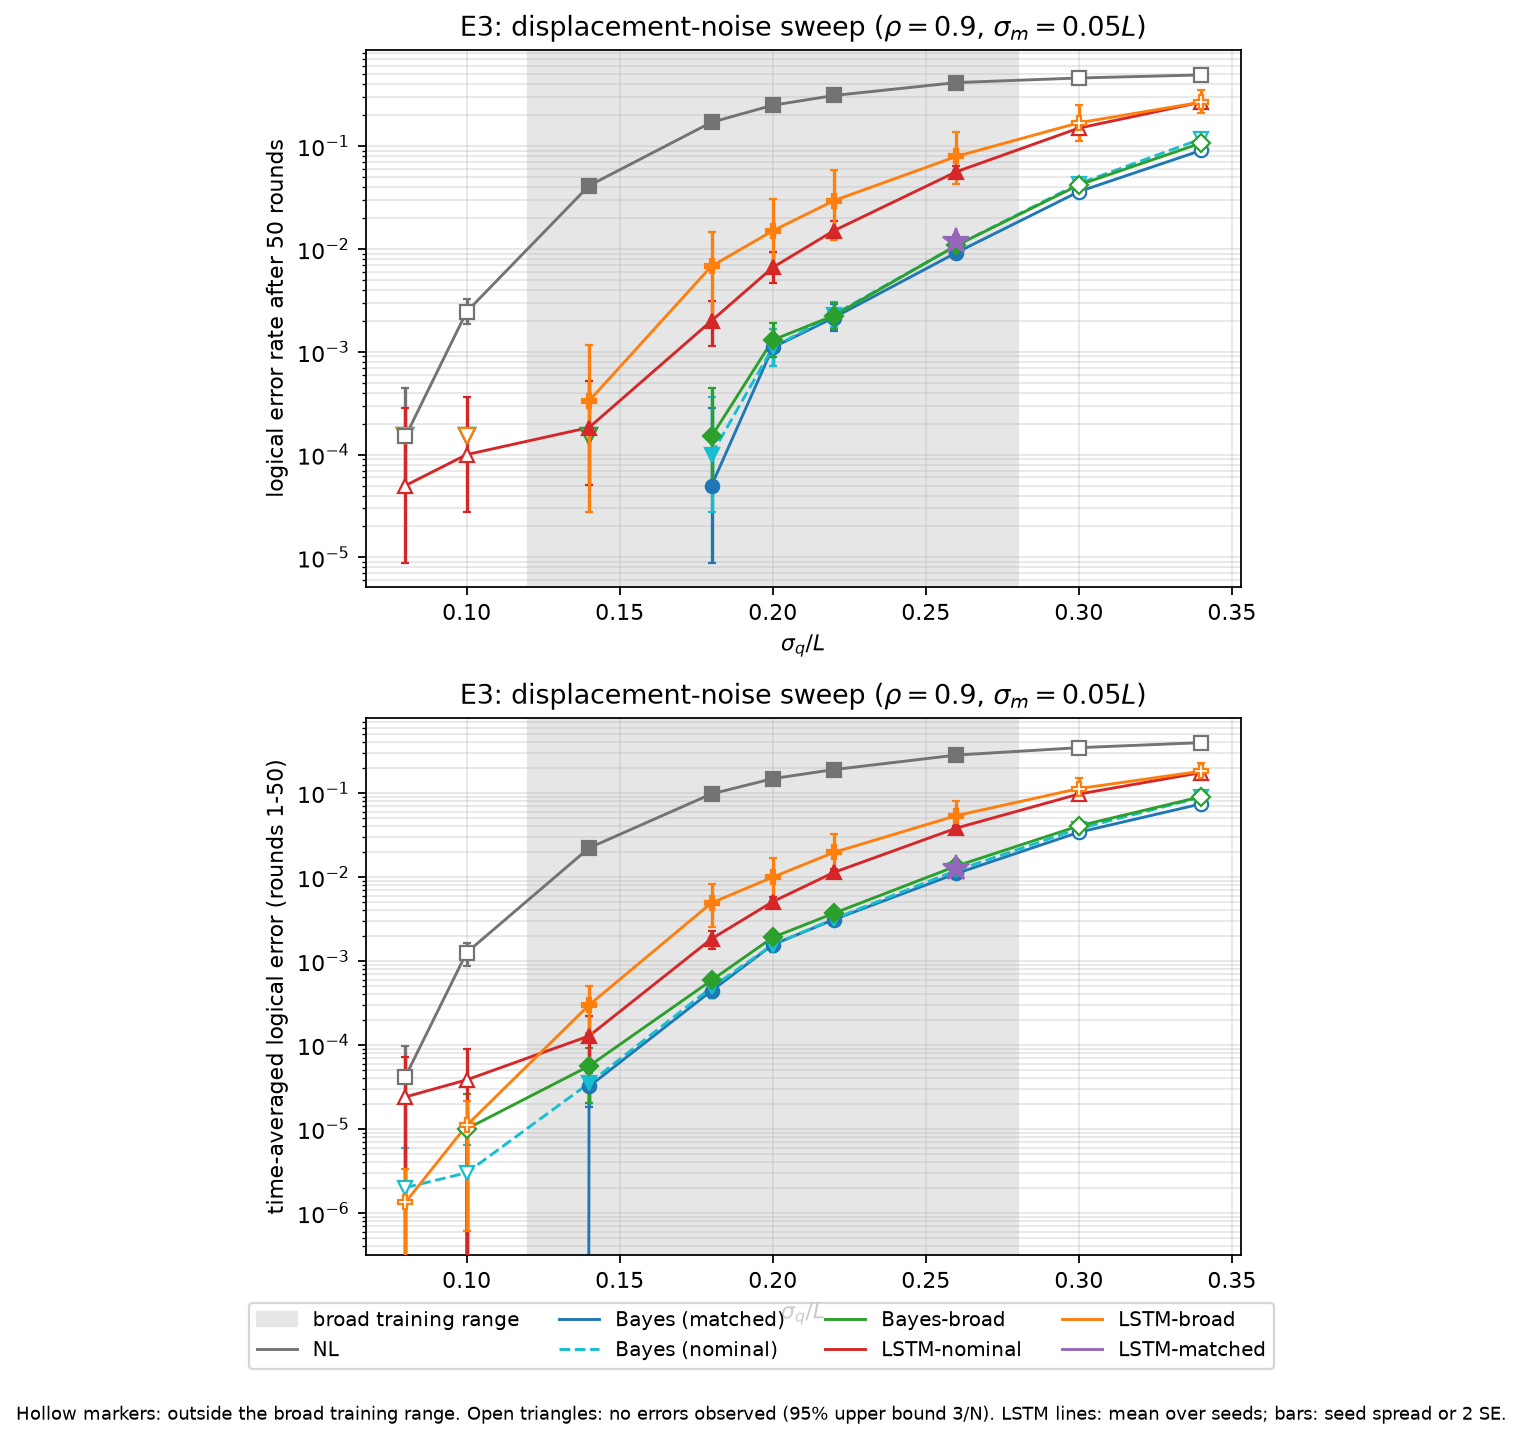
\includegraphics[width=0.95\textwidth]{E3_sigma_q_sweep.png}
\caption{E3: displacement-noise sweep at $\rho=0.9$, $\sigma_m=0.05L$.}
\label{fig:e3}
\end{figure}

\begin{figure}[H]
\centering
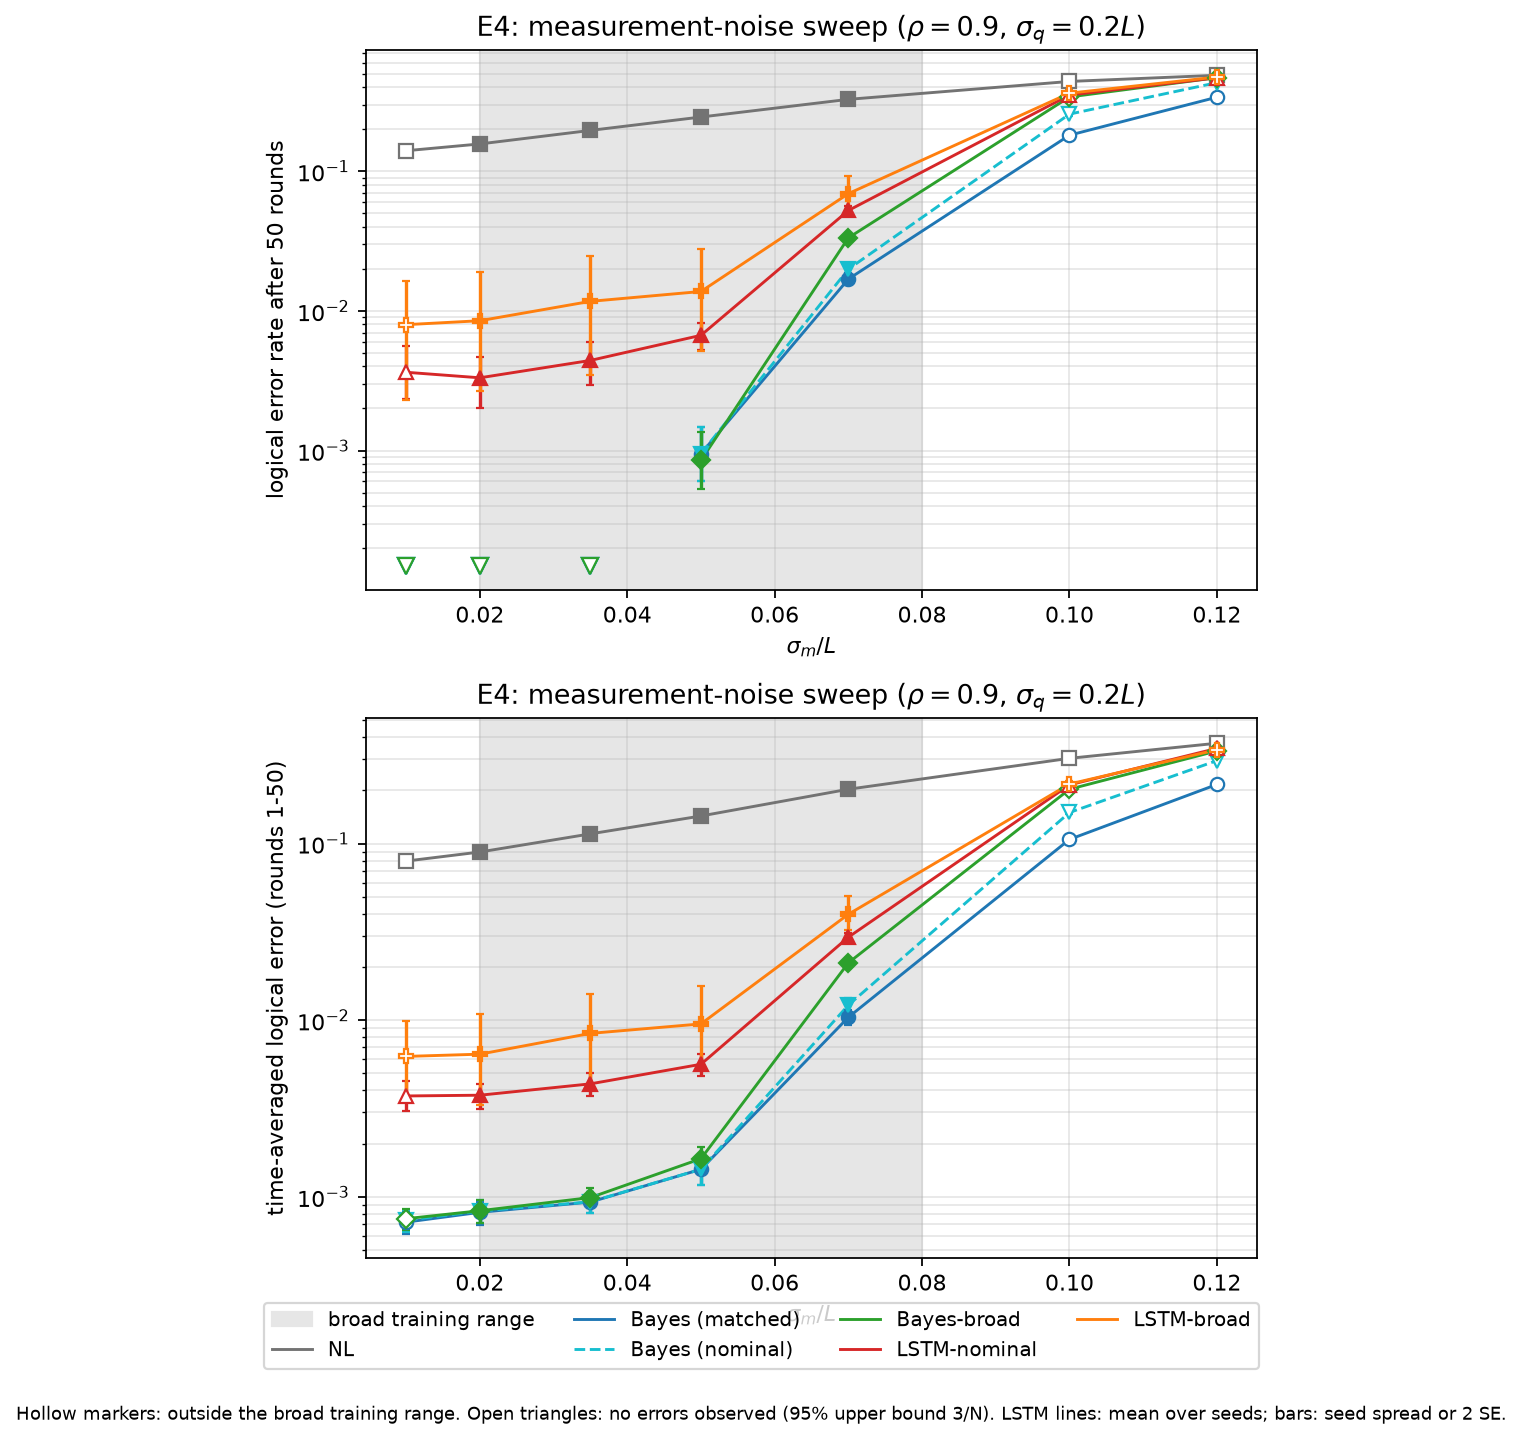
\includegraphics[width=0.95\textwidth]{E4_sigma_m_sweep.png}
\caption{E4: measurement-noise sweep at $\rho=0.9$, $\sigma_q=0.2L$.}
\label{fig:e4}
\end{figure}

\begin{table}[H]
\centering\small
\resizebox{\textwidth}{!}{\begin{tabular}{lrrrrrrr}
\toprule
$\sigma_q/L$ & NL & Bayes (matched) & Bayes (nominal) & Bayes-broad & LSTM-nominal & LSTM-broad & LSTM-matched \\
\midrule
0.08 & $1.5\!\times\!10^{-4}$$^\dagger$ & $<1.5\!\times\!10^{-4}$ & $<1.5\!\times\!10^{-4}$ & \textit{$<1.5\!\times\!10^{-4}$} & $5.0\!\times\!10^{-5}$$^\dagger$ & \textit{$<1.5\!\times\!10^{-4}$} & -- \\
0.1 & $2.4\!\times\!10^{-3}$ & $<1.5\!\times\!10^{-4}$ & $<1.5\!\times\!10^{-4}$ & \textit{$<1.5\!\times\!10^{-4}$} & $1.0\!\times\!10^{-4}$$^\dagger$ & \textit{$<1.5\!\times\!10^{-4}$} & -- \\
0.14 & $0.041$ & $<1.5\!\times\!10^{-4}$ & $<1.5\!\times\!10^{-4}$ & $<1.5\!\times\!10^{-4}$ & $1.8\!\times\!10^{-4}$ & $3.3\!\times\!10^{-4}$ & -- \\
0.18 & $0.170$ & $5.0\!\times\!10^{-5}$$^\dagger$ & $1.0\!\times\!10^{-4}$$^\dagger$ & $1.5\!\times\!10^{-4}$$^\dagger$ & $2.0\!\times\!10^{-3}$ & $6.8\!\times\!10^{-3}$ & -- \\
0.2 & $0.249$ & $1.1\!\times\!10^{-3}$ & $1.1\!\times\!10^{-3}$ & $1.3\!\times\!10^{-3}$ & $6.6\!\times\!10^{-3}$ & $0.015$ & -- \\
0.22 & $0.310$ & $2.1\!\times\!10^{-3}$ & $2.3\!\times\!10^{-3}$ & $2.2\!\times\!10^{-3}$ & $0.015$ & $0.029$ & -- \\
0.26 & $0.414$ & $9.2\!\times\!10^{-3}$ & $0.011$ & $0.011$ & $0.056$ & $0.079$ & $0.012$ \\
0.3 & $0.459$ & $0.036$ & $0.043$ & \textit{$0.042$} & $0.150$ & \textit{$0.168$} & -- \\
0.34 & $0.492$ & $0.091$ & $0.117$ & \textit{$0.107$} & $0.268$ & \textit{$0.267$} & -- \\
\bottomrule
\end{tabular}}
\\[4pt]
\resizebox{0.9\textwidth}{!}{\begin{tabular}{lrrrrrr}
\toprule
$\sigma_m/L$ & NL & Bayes (matched) & Bayes (nominal) & Bayes-broad & LSTM-nominal & LSTM-broad \\
\midrule
0.01 & $0.140$ & $<1.5\!\times\!10^{-4}$ & $<1.5\!\times\!10^{-4}$ & \textit{$<1.5\!\times\!10^{-4}$} & $3.6\!\times\!10^{-3}$ & \textit{$8.0\!\times\!10^{-3}$} \\
0.02 & $0.157$ & $<1.5\!\times\!10^{-4}$ & $<1.5\!\times\!10^{-4}$ & $<1.5\!\times\!10^{-4}$ & $3.3\!\times\!10^{-3}$ & $8.5\!\times\!10^{-3}$ \\
0.035 & $0.196$ & $<1.5\!\times\!10^{-4}$ & $<1.5\!\times\!10^{-4}$ & $<1.5\!\times\!10^{-4}$ & $4.4\!\times\!10^{-3}$ & $0.012$ \\
0.05 & $0.244$ & $9.5\!\times\!10^{-4}$ & $9.5\!\times\!10^{-4}$ & $8.5\!\times\!10^{-4}$ & $6.7\!\times\!10^{-3}$ & $0.014$ \\
0.07 & $0.327$ & $0.017$ & $0.020$ & $0.033$ & $0.052$ & $0.069$ \\
0.1 & $0.440$ & $0.181$ & $0.257$ & \textit{$0.340$} & $0.351$ & \textit{$0.362$} \\
0.12 & $0.487$ & $0.339$ & $0.431$ & \textit{$0.468$} & $0.467$ & \textit{$0.473$} \\
\bottomrule
\end{tabular}}
\caption{E3 (top) and E4 (bottom): $P_L(50)$; 20{,}000 trials per point.}
\label{tab:e34}
\end{table}

\paragraph{Displacement noise.}
All errors rise steeply with $\sigma_q$ (Figure~\ref{fig:e3}). Wherever
errors are resolved ($\sigma_q\ge0.14L$), the ordering of the nominal and
broad decoders never changes: matched Bayes is best, then Bayes (nominal) and
Bayes-broad, then LSTM-nominal and LSTM-broad, then NL. The exception is the
LSTM trained at $\sigma_q=0.26L$, which is level with the model-based filters
at that point. The model-based filters are remarkably
insensitive to a wrong $\sigma_q$ here. Bayes (nominal) assumes
$\sigma_q=0.2L$ and is within 20\% of matched Bayes up to $\sigma_q=0.34L$.

At $\sigma_q=0.26L$ the matched LSTM (error
$\res{E3}{sq0.26}{LSTM-matched}$) is again close to matched Bayes
($\resratio{E3}{sq0.26}{LSTM-matched}\times$). LSTM-nominal is
$\resratio{E3}{sq0.26}{LSTM-nominal}\times$ matched Bayes at that point.

\paragraph{Measurement noise.}
Measurement noise is the harder axis (Figure~\ref{fig:e4}). Once $\sigma_m$
reaches about $0.07L$, the syndrome no longer pins down the error well, and
every decoder degrades quickly. At $\sigma_m=0.10L$:
\begin{itemize}
  \item Bayes (nominal), which assumes $\sigma_m=0.05L$, has error
    $\res{E4}{sm0.1}{Bayes (nominal)}$, against
    $\res{E4}{sm0.1}{Bayes (matched)}$ for matched Bayes.
  \item Bayes-broad, whose components all assume $\sigma_m'=0.05L$, has error
    $\res{E4}{sm0.1}{Bayes-broad}$. That is still about 6\% better than the
    LSTMs (LSTM-broad $\res{E4}{sm0.1}{LSTM-broad}$, LSTM-nominal
    $\res{E4}{sm0.1}{LSTM-nominal}$), but most of its earlier lead is gone.
\end{itemize}

%----------------------------------------
\subsection{E5: Bayes with a mis-specified model}

\begin{figure}[H]
\centering
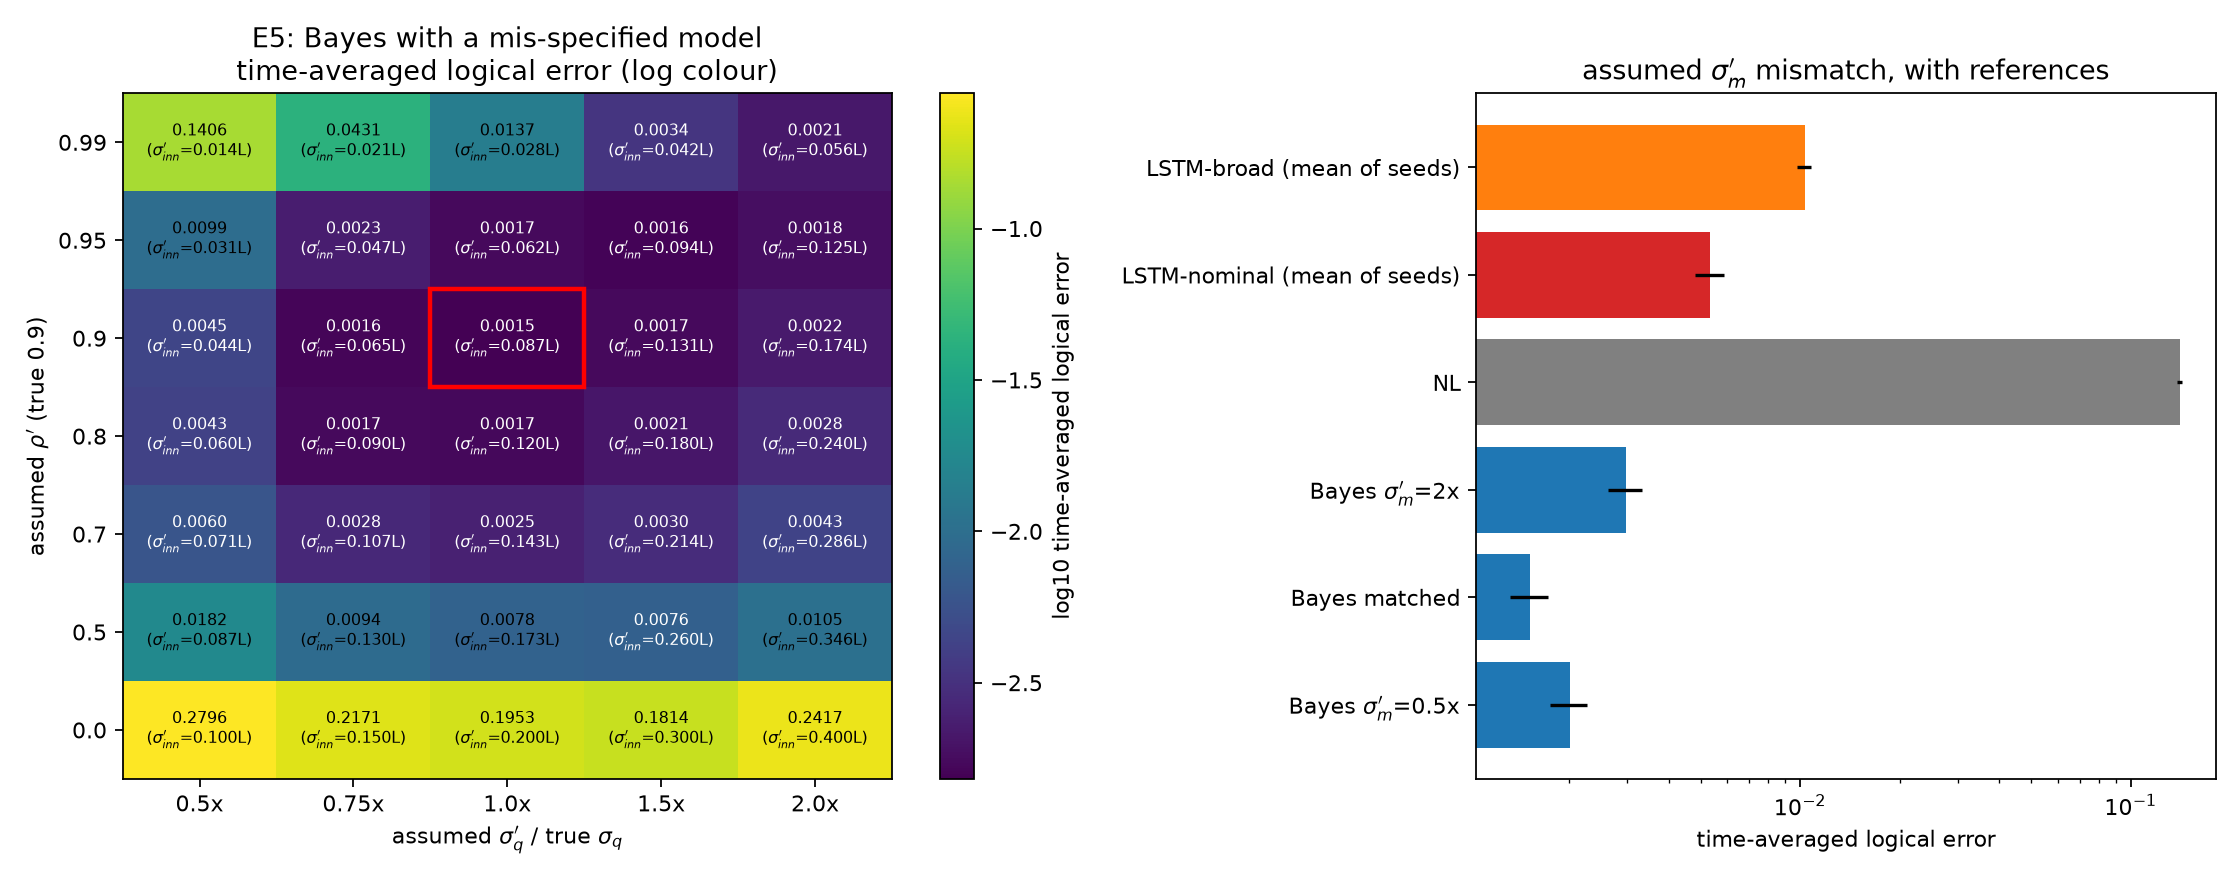
\includegraphics[width=\textwidth]{E5_mismatch.png}
\caption{E5: time-averaged error of Bayes filters with wrong assumed
parameters, at the nominal truth (\EfiveTrials{} trials, common noise). Each
cell gives the innovation standard deviation implied by the assumed
parameters; the true value is $0.087L$ (red box).}
\label{fig:e5}
\end{figure}

\begin{table}[H]
\centering\small
\begin{tabular}{lrrrrr}
\toprule
$\rho'$ \textbackslash{} $\sigma_q'/\sigma_q$ & 0.5 & 0.75 & 1.0 & 1.5 & 2.0 \\
\midrule
0.0 & $0.280$ & $0.217$ & $0.195$ & $0.181$ & $0.242$ \\
0.5 & $0.018$ & $9.4\!\times\!10^{-3}$ & $7.8\!\times\!10^{-3}$ & $7.6\!\times\!10^{-3}$ & $0.010$ \\
0.7 & $6.0\!\times\!10^{-3}$ & $2.8\!\times\!10^{-3}$ & $2.5\!\times\!10^{-3}$ & $3.0\!\times\!10^{-3}$ & $4.3\!\times\!10^{-3}$ \\
0.8 & $4.3\!\times\!10^{-3}$ & $1.7\!\times\!10^{-3}$ & $1.7\!\times\!10^{-3}$ & $2.1\!\times\!10^{-3}$ & $2.8\!\times\!10^{-3}$ \\
0.9 & $4.5\!\times\!10^{-3}$ & $1.6\!\times\!10^{-3}$ & \textbf{$1.5\!\times\!10^{-3}$} & $1.7\!\times\!10^{-3}$ & $2.2\!\times\!10^{-3}$ \\
0.95 & $9.9\!\times\!10^{-3}$ & $2.3\!\times\!10^{-3}$ & $1.7\!\times\!10^{-3}$ & $1.6\!\times\!10^{-3}$ & $1.8\!\times\!10^{-3}$ \\
0.99 & $0.141$ & $0.043$ & $0.014$ & $3.4\!\times\!10^{-3}$ & $2.1\!\times\!10^{-3}$ \\
\bottomrule
\end{tabular}
\caption{E5: time-averaged error against the assumed $\rho'$ (rows) and
$\sigma_q'/\sigma_q$ (columns). The truth is $\rho=0.9$; the matched cell is
in bold.}
\label{tab:e5}
\end{table}

The filter tolerates moderate mismatch well. Every model with
$0.8\le\rho'\le0.95$ and $0.75\le\sigma_q'/\sigma_q\le1.5$ stays within
$1.6\times$ of the matched error. Near the true correlation, the assumed
innovation standard deviation $\sigma_q'\sqrt{1-\rho'^2}$ (printed in each
cell) is a useful guide, but it does not determine the error by itself:
\begin{itemize}
  \item \textbf{Overestimating it by raising $\sigma_q'$ is cheap.} With
    $\sigma_q'=2\sigma_q$ the error only rises to $\EfiveSqTwoMean$. Getting
    a similar overestimate by lowering $\rho'$ costs much more: $\rho'=0.5$
    gives $\EfiveRhoHalfMean$.
  \item \textbf{Underestimating it is expensive.} A filter that thinks the
    displacement is more predictable than it is becomes overconfident. With
    $\rho'=0.99$ the error is $\EfiveRhoHighMean$; with $\rho'=0.99$ and
    $\sigma_q'=0.5\sigma_q$ it collapses to NL's level
    ($\res{E5}{nominal}{Bayes rho'=0.99 sq'x0.5}$).
  \item \textbf{Assuming no correlation ($\rho'=0$)} is worse than NL
    ($\EfiveRhoZeroMean$ against $\EfiveNLMean$). The filter then commits to
    the wrong cell whenever the current syndrome is ambiguous, and it never
    uses the history that would have resolved it.
  \item \textbf{A wrong measurement noise} costs up to about a factor of 2
    at the two values tested ($\sigma_m'=0.5\sigma_m$: $\EfiveSmHalfMean$;
    $\sigma_m'=2\sigma_m$: $\EfiveSmTwoMean$).
\end{itemize}
Measured against this scale, LSTM-nominal ($\EfiveLSTMnomMean$, at its own
training point) is about as good as a Bayes filter with a moderately wrong
model, e.g.\ $\rho'=0.7$ and $\sigma_q'=0.5\sigma_q$. Many mis-specified
filters beat it, and some severely mis-specified ones do not.

%----------------------------------------
\subsection{E6: regime-switching noise}

\begin{figure}[H]
\centering
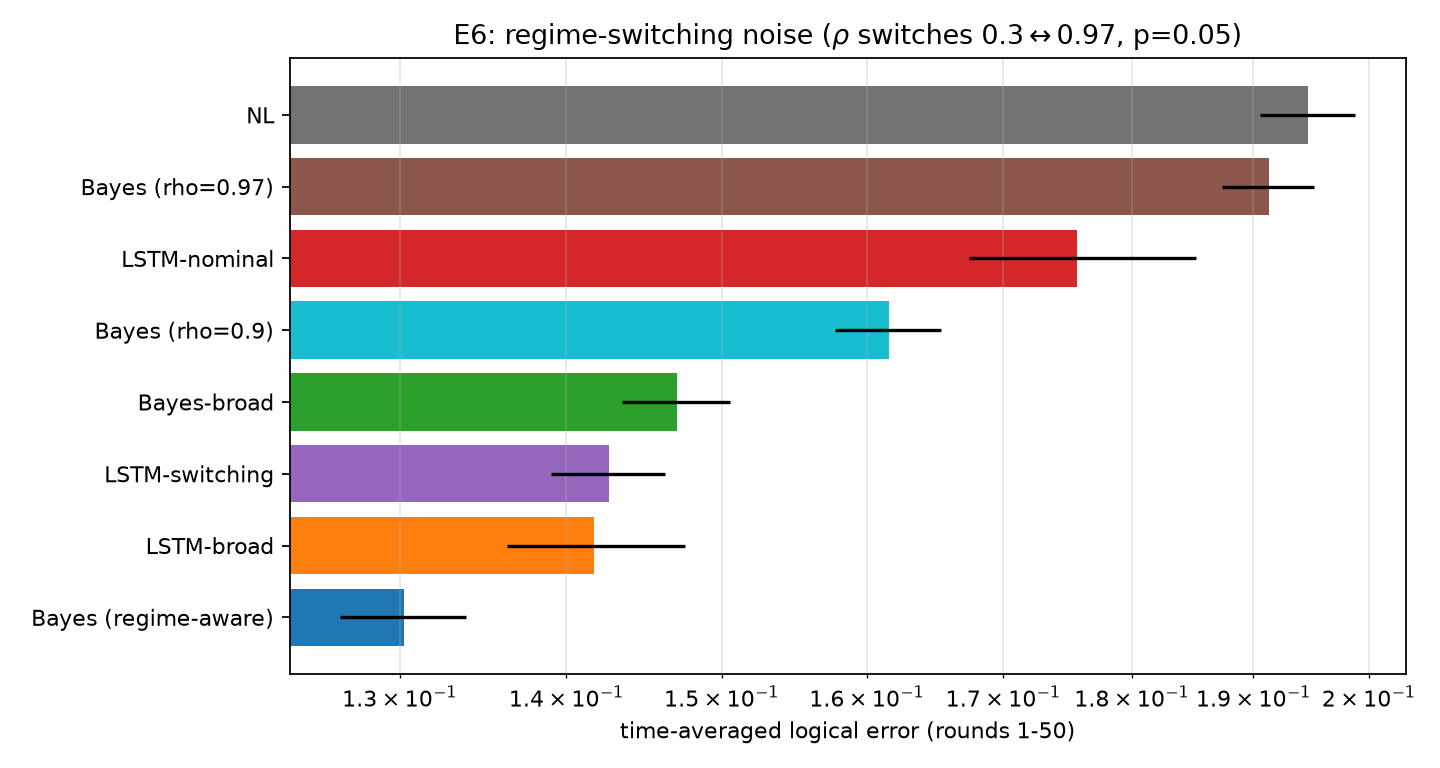
\includegraphics[width=0.75\textwidth]{E6_switching.png}
\caption{E6: the correlation switches between $\rho=0.3$ and $\rho=0.97$ with
probability 0.05 per round. Bars show the 2-SE test-noise uncertainty plus,
for the LSTM seed means, the spread between seeds.}
\label{fig:e6}
\end{figure}

\begin{table}[H]
\centering\small
\begin{tabular}{lrrr}
\toprule
Decoder & $P_L(10)$ & $P_L(50)$ & time-avg.\ error \\
\midrule
NL & $0.101$ & $0.320$ & $0.195$ \\
Bayes (regime-aware) & $0.061$ & $0.226$ & $0.130$ \\
Bayes (rho=0.9) & $0.081$ & $0.269$ & $0.162$ \\
Bayes (rho=0.97) & $0.099$ & $0.312$ & $0.191$ \\
Bayes-broad & $0.065$ & $0.251$ & $0.147$ \\
LSTM-nominal (mean of seeds) & $0.091$ & $0.290$ & $0.176$ {\scriptsize[0.17,\,0.18]} \\
LSTM-broad (mean of seeds) & $0.065$ & $0.246$ & $0.142$ {\scriptsize[0.14,\,0.14]} \\
LSTM-switching & $0.068$ & $0.247$ & $0.143$ \\
\bottomrule
\end{tabular}
\caption{E6: switching noise (20{,}000 trials, common noise).}
\label{tab:e6}
\end{table}

Under noise whose correlation switches between regimes, the decoder that
models the switching is best: regime-aware Bayes has error
$\EsixBayesregimeawareMean$, against $\EsixNLMean$ for NL. This is the
setting where the proposal expected machine learning to help when the
Bayesian model is wrong, and it does. LSTM-broad ($\EsixLSTMbroadMean$) beats
every \emph{fixed-model} Bayes filter:
\begin{itemize}
  \item $\rho=0.9$: $\EsixBayesrhozeronineMean$;
  \item $\rho=0.97$: $\EsixBayesrhozeroninesevenMean$, worse than LSTM-nominal;
  \item Bayes-broad: $\EsixBayesbroadMean$.
\end{itemize}
An LSTM trained on the switching noise itself ($\EsixLSTMswitchingMean$) is
no better than the broad one. So the LSTM's advantage over the fixed filters
here comes from having seen varied correlations, not from learning this
specific process.

%----------------------------------------
\subsection{E7: computational cost}

\begin{table}[H]
\centering\small
\begin{tabular}{llrrr}
\toprule
Decoder & device & batch & ms / round & trial-rounds / s \\
\midrule
Bayes (matched) & cuda & 1 & 3.43 & 292 \\
Bayes (matched) & cuda & 4096 & 13.3 & 3.08e+05 \\
Bayes-broad & cuda & 1 & 22.6 & 44.2 \\
Bayes-broad & cuda & 4096 & 122 & 3.36e+04 \\
LSTM-nominal s0 & cuda & 1 & 1.5 & 668 \\
LSTM-nominal s0 & cuda & 4096 & 13 & 3.15e+05 \\
NL & cpu & 1 & 0.00644 & 1.55e+05 \\
NL & cpu & 512 & 0.0188 & 2.72e+07 \\
Bayes (matched) & cpu & 1 & 0.873 & 1.15e+03 \\
Bayes (matched) & cpu & 512 & 53.1 & 9.65e+03 \\
Bayes-broad & cpu & 1 & 4.77 & 210 \\
Bayes-broad & cpu & 512 & 437 & 1.17e+03 \\
LSTM-nominal s0 & cpu & 1 & 0.944 & 1.06e+03 \\
LSTM-nominal s0 & cpu & 512 & 1.93 & 2.66e+05 \\
\bottomrule
\end{tabular}
\caption{E7: decoding cost per round, measured on an otherwise idle
\GPUname{} and the host CPU. Batch 1 gives the latency of one decoder instance;
the large batch gives throughput.}
\label{tab:e7}
\end{table}

For a single trial on the CPU, NL takes microseconds, while matched Bayes and
the LSTM both take about a millisecond per round
($\tim{Bayes (matched)}{cpu}{1}{latency}$ and
$\tim{LSTM-nominal s0}{cpu}{1}{latency}$~ms). Batched, the picture differs by
device:
\begin{itemize}
  \item \textbf{GPU:} the LSTM and the grid filter have similar throughput
    ($\tim{LSTM-nominal s0}{cuda}{4096}{throughput}$ against
    $\tim{Bayes (matched)}{cuda}{4096}{throughput}$ trial-rounds/s).
  \item \textbf{CPU:} the LSTM's throughput is about 27 times the filter's.
\end{itemize}
Batched, Bayes-broad (8 components) costs as much as 8--9 single filters; for
a single trial it costs about 5.5--6.6 times one filter. Training each LSTM
took 6--11~minutes of wall time for 40 epochs, measured while the GPU was
shared with the Bayes evaluations (Table~\ref{tab:training}). The filter's cost grows with
the grid ($n_x\times n_\varepsilon$ cells per trial) and would grow further
with more hidden variables, e.g.\ for regimes or the $p$ quadrature. The
LSTM's cost is fixed by its size.
